% begin module natural-exponential-intro
\begin{frame}
\frametitle{The Natural Exponential Function}
\begin{itemize}
\item  One base for an exponential function is especially useful.
\item<2->  It has a special property: its tangent line at $x = 0$ has slope $m=1$.
\item<3->  We call this number $e$, known as Euler's number or Napier's constant.
\item<4->  $e$ is a number between 2 and 3.  
\item<5-> In fact, $e = 1+1+\frac{1}{2!}+\frac{1}{3!} +\frac{1}{4!}+\dots\approx 2.71828$.  
\end{itemize}

\begin{columns}
\column{.3\textwidth}
\psset{xunit=1.3cm, yunit=1.3cm}
\begin{pspicture}(-5, -5)(5,5) 
\psframe*[linecolor=white](-5,-5)(5,5) 
\psaxes[labels=none]{<->}(0,0)(-1.3, -0.5)(1.3,2.5)
\psplot[linecolor=red, plotpoints=1000]{-1.3}{1.3}{2 x exp}
\rput[r](-0.2, 1.1){\footnotesize $y=2^x$}
\rput[l](0.2, 0.8){\tiny $m\approx 0.693147$} 
\psline[linecolor=blue](-1.3,0.098908665)(1.3, 1.901091335)
\end{pspicture}
%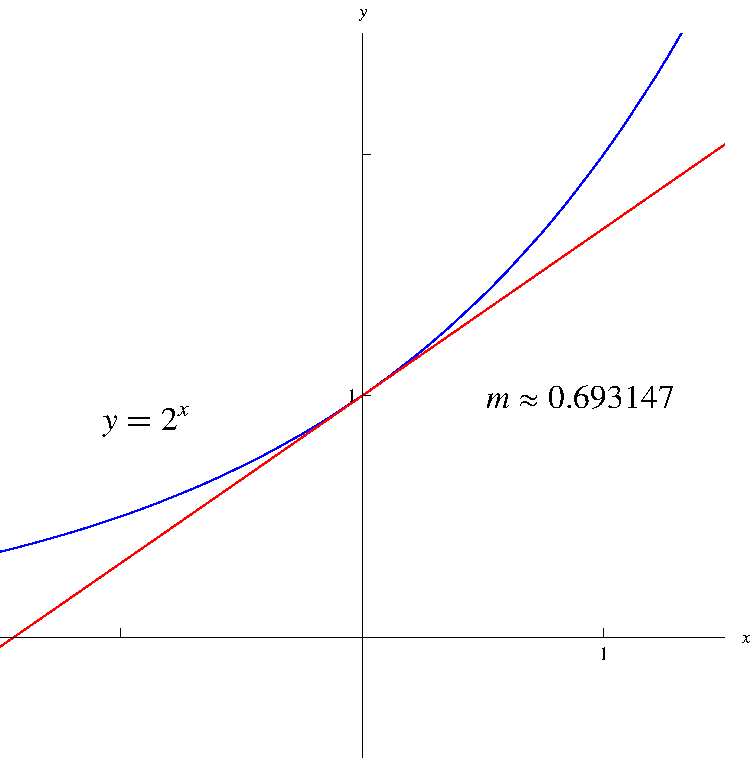
\includegraphics[height=4cm]{exponential-functions/pictures/exp-tangent-two.pdf}%
\column{.3\textwidth}
\uncover<handout: 1|3->{%
\psset{xunit=1.3cm, yunit=1.3cm}
\begin{pspicture}(-5, -5)(5,5) 
\psframe*[linecolor=white](-5,-5)(5,5) 
\psaxes[labels=none]{<->}(0,0)(-1.3, -0.5)(1.3,2.5)
\psplot[linecolor=red, plotpoints=1000]{-1.3}{0.901091335}{2.718281828 x exp}
\rput[r](-0.2, 1.1){\footnotesize $y=e^x$}
\rput[l](0.2, 0.8){\tiny $m=1$}
\psline[linecolor=blue](-1.3, -0.3)(1.3,2.3) 
\end{pspicture}
%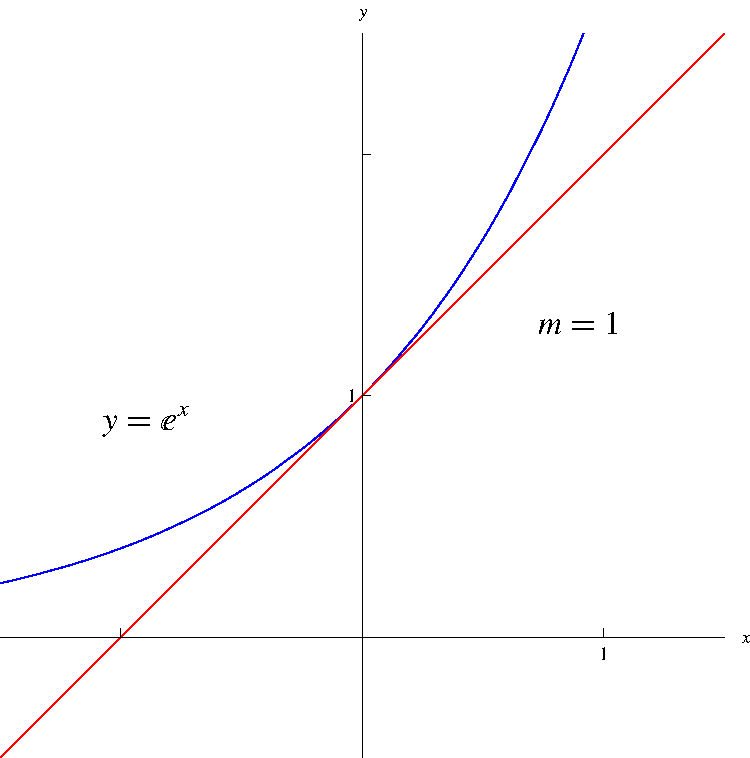
\includegraphics[height=4cm]{exponential-functions/pictures/exp-tangent-e.pdf}%
}%
\column{.3\textwidth}
\psset{xunit=1.3cm, yunit=1.3cm}
\begin{pspicture}(-5, -5)(5,5) 
\psframe*[linecolor=white](-5,-5)(5,5) 
\psaxes[labels=none]{<->}(0,0)(-1.3, -0.5)(1.3,2.5)
\psplot[linecolor=red, plotpoints=1000]{-1.3}{0.82020868}{3 x exp}
\rput[r](-0.2, 1.1){\footnotesize $y=3^x$}
\rput[l](0.2, 0.8){\tiny $m\approx 1.09861$} 
\psline[linecolor=blue](-1.3, -0.428195975)(1.3,2.428195975)
\end{pspicture}
%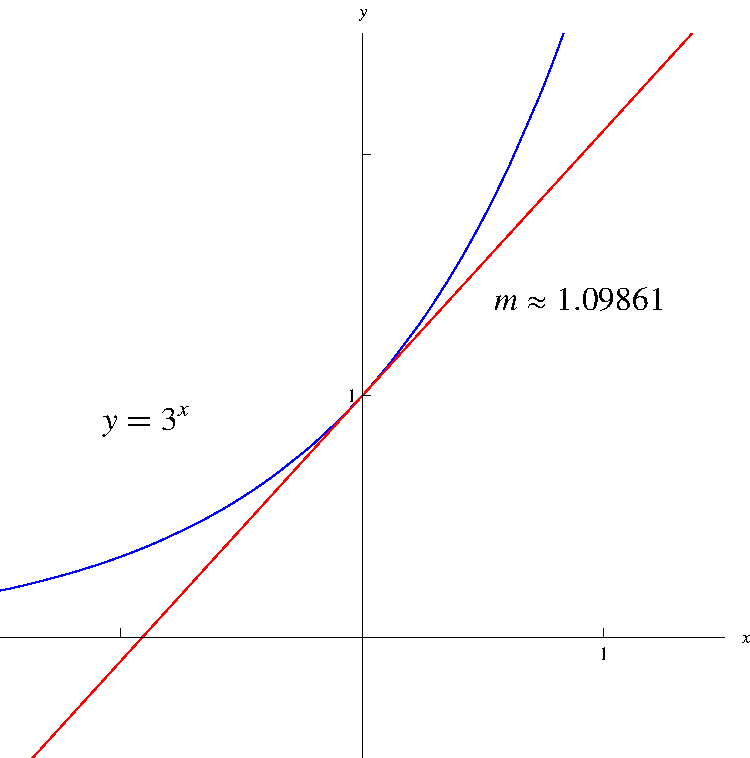
\includegraphics[height=4cm]{exponential-functions/pictures/exp-tangent-three.pdf}%
\end{columns}
\end{frame}
% end module natural-exponential-intro